
\documentclass[border=18pt, multi, tikz]{standalone}
\usepackage{import}
\usepackage{graphicx}
\subimport{layers/}{init}

\usetikzlibrary{positioning}
\usetikzlibrary{3d}
\usetikzlibrary{calc}
\usetikzlibrary{patterns}


%%%%%%%%%%%%%%%%%%%%%%%%%%%%%%%%%%%%%%%%%%%%%%%%%%%%%%%%%%%%%%%%%%%%%%%%%%%%%%%%%%%%%%%%
%% COLORS
%%%%%%%%%%%%%%%%%%%%%%%%%%%%%%%%%%%%%%%%%%%%%%%%%%%%%%%%%%%%%%%%%%%%%%%%%%%%%%%%%%%%%%%%
%% color definitions used throughout the CNN architecture visualization
%% separate colors are used for convolution blocks, pooling, dense layers,
%% activations and prediction/output elements
%%%%%%%%%%%%%%%%%%%%%%%%%%%%%%%%%%%%%%%%%%%%%%%%%%%%%%%%%%%%%%%%%%%%%%%%%%%%%%%%%%%%%%%%

\def\ConvColor{rgb:yellow,5;red,2.5;white,5}
\def\ConvReluColor{rgb:yellow,5;red,5;white,5}

\def\InputColor{rgb:blue,2.5;gray,4;white,5}
\def\InputBandColor{rgb:yellow,5;red,5;white,5}

\def\PoolColor{rgb:red,1;black,0.3}
\def\GapColor{rgb:red,1;black,0.15;white,0.8}

\def\FcColor{rgb:blue,5;red,2.5;white,5}
\def\FcReluColor{rgb:blue,5;red,5;white,1}

\def\DropoutColor{rgb:black,4.7;white,7}

\def\SoftmaxColor{rgb:magenta,5;black,7}
\def\SoftmaxBandColor{rgb:magenta,5;black,4}

\def\edgecolor{rgb:green,4;blue,1.5;red,0.5;black,3.8}
\definecolor{PredictionGreen}{RGB}{120,190,120}

\begin{document}

\begin{tikzpicture}

%%%%%%%%%%%%%%%%%%%%%%%%%%%%%%%%%%%%%%%%%%%%%%%%%%%%%%%%%%%%%%%%%%%%%%%%%%%%%%%%%%%%%%%%
%% CONNECTION STYLE
%%%%%%%%%%%%%%%%%%%%%%%%%%%%%%%%%%%%%%%%%%%%%%%%%%%%%%%%%%%%%%%%%%%%%%%%%%%%%%%%%%%%%%%%
%% defines the appearance of the forward data flow arrows
%% between CNN layers
%%%%%%%%%%%%%%%%%%%%%%%%%%%%%%%%%%%%%%%%%%%%%%%%%%%%%%%%%%%%%%%%%%%%%%%%%%%%%%%%%%%%%%%%

\tikzstyle{connection}=[
    line width=2.2pt,
    every node/.style={sloped,allow upside down},
    draw=\edgecolor,
    opacity=0.75
]

%%%%%%%%%%%%%%%%%%%%%%%%%%%%%%%%%%%%%%%%%%%%%%%%%%%%%%%%%%%%%%%%%%%%%%%%%%%%%%%%%%%%%%%%
%% RAW IMAGE
%%%%%%%%%%%%%%%%%%%%%%%%%%%%%%%%%%%%%%%%%%%%%%%%%%%%%%%%%%%%%%%%%%%%%%%%%%%%%%%%%%%%%%%%
%% original input image before resizing and preprocessing
%%%%%%%%%%%%%%%%%%%%%%%%%%%%%%%%%%%%%%%%%%%%%%%%%%%%%%%%%%%%%%%%%%%%%%%%%%%%%%%%%%%%%%%%

\node[canvas is zy plane at x=0] (rawinput) at (-5.2,0,0)
{
    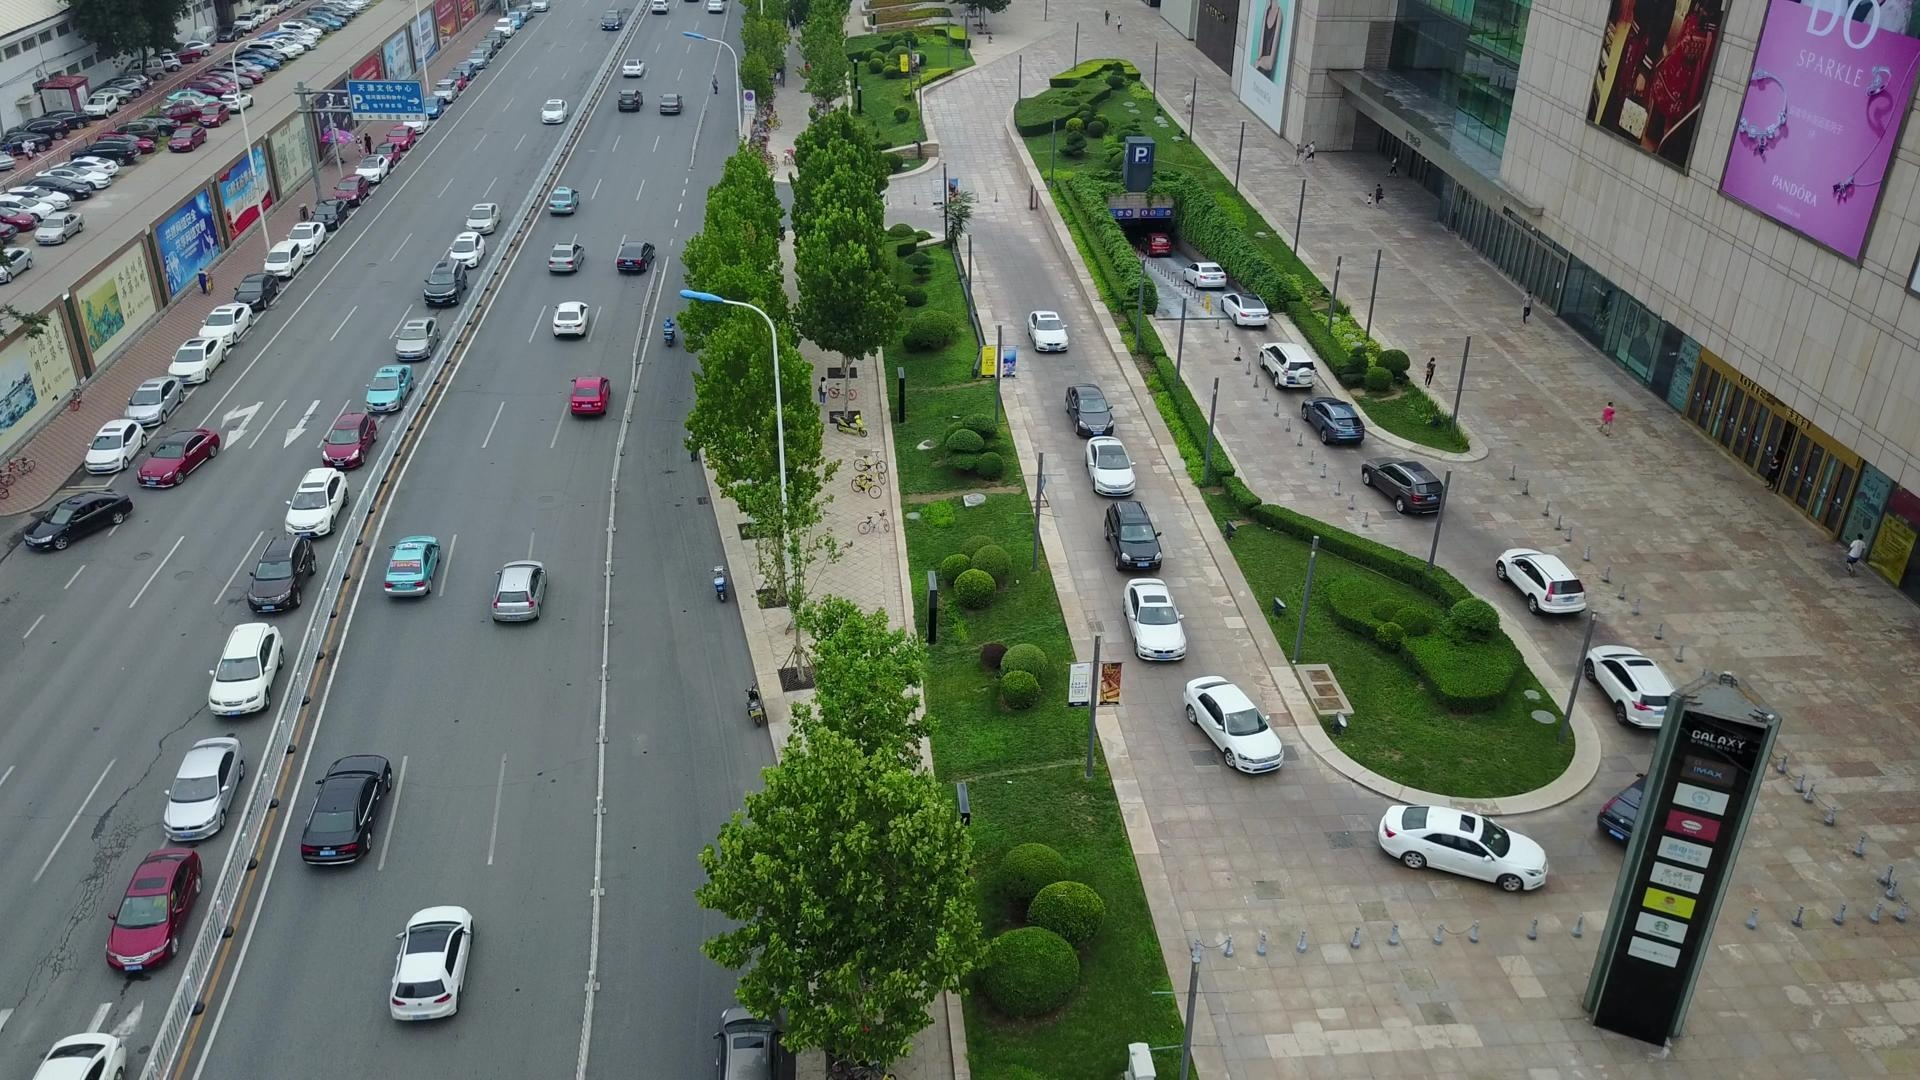
\includegraphics[width=18cm,keepaspectratio]{sample_input.jpg}
};


%%%%%%%%%%%%%%%%%%%%%%%%%%%%%%%%%%%%%%%%%%%%%%%%%%%%%%%%%%%%%%%%%%%%%%%%%%%%%%%%%%%%%%%%
%% RAW IMAGE CORNERS
%%%%%%%%%%%%%%%%%%%%%%%%%%%%%%%%%%%%%%%%%%%%%%%%%%%%%%%%%%%%%%%%%%%%%%%%%%%%%%%%%%%%%%%%
%% helper coordinates used for resize projection lines
%%
%% width=18cm
%% aspect ratio = 1360x768
%%
%% half width  = 9
%% half height = 18 * (768/1360) / 2 = 5.08
%%%%%%%%%%%%%%%%%%%%%%%%%%%%%%%%%%%%%%%%%%%%%%%%%%%%%%%%%%%%%%%%%%%%%%%%%%%%%%%%%%%%%%%%

\coordinate (raw-nw) at (-5.2,  5.08, -9);
\coordinate (raw-ne) at (-5.2,  5.08,  9);
\coordinate (raw-sw) at (-5.2, -5.08, -9);
\coordinate (raw-se) at (-5.2, -5.08,  9);

%%%%%%%%%%%%%%%%%%%%%%%%%%%%%%%%%%%%%%%%%%%%%%%%%%%%%%%%%%%%%%%%%%%%%%%%%%%%%%%%%%%%%%%%
%% RAW IMAGE LABEL
%%%%%%%%%%%%%%%%%%%%%%%%%%%%%%%%%%%%%%%%%%%%%%%%%%%%%%%%%%%%%%%%%%%%%%%%%%%%%%%%%%%%%%%%
%% label for original input image resolution
%%%%%%%%%%%%%%%%%%%%%%%%%%%%%%%%%%%%%%%%%%%%%%%%%%%%%%%%%%%%%%%%%%%%%%%%%%%%%%%%%%%%%%%%

\path
(raw-sw) -- (raw-se)
node[
    midway,
    below=0.1cm,
    sloped,
    align=center
]
{
    \bfseries ~~~~~~~~raw input image\\[-1mm]
    \ ~~~~~~~~1360 $\times$ 768 px
};

%%%%%%%%%%%%%%%%%%%%%%%%%%%%%%%%%%%%%%%%%%%%%%%%%%%%%%%%%%%%%%%%%%%%%%%%%%%%%%%%%%%%%%%%
%% INPUT TENSOR
%%%%%%%%%%%%%%%%%%%%%%%%%%%%%%%%%%%%%%%%%%%%%%%%%%%%%%%%%%%%%%%%%%%%%%%%%%%%%%%%%%%%%%%%
%% CNN input tensor after resizing to fixed 128 x 128 RGB
%%%%%%%%%%%%%%%%%%%%%%%%%%%%%%%%%%%%%%%%%%%%%%%%%%%%%%%%%%%%%%%%%%%%%%%%%%%%%%%%%%%%%%%%

\pic[shift={(0,0,0)}] at (0,0,0)
{Box={
    name=input,
    fill=\InputColor,
    opacity=0.6,
    height=40,
    width=1,
    depth=40,
    xlabel={{"3~",""}},
    zlabel=~~128,
    hideedgex=1,
    hideedgey=1,
    hideedgez=1
}};


\node[shift={(-1.85cm,-5.35cm)}] at (input-west)
{
    \small 128
};


%%%%%%%%%%%%%%%%%%%%%%%%%%%%%%%%%%%%%%%%%%%%%%%%%%%%%%%%%%%%%%%%%%%%%%%%%%%%%%%%%%%%%%%%
%% RESIZED IMAGE ON INPUT FACE
%%%%%%%%%%%%%%%%%%%%%%%%%%%%%%%%%%%%%%%%%%%%%%%%%%%%%%%%%%%%%%%%%%%%%%%%%%%%%%%%%%%%%%%%
%% resized RGB image projected directly onto the input tensor
%% to visually connect preprocessing and CNN input representation
%%%%%%%%%%%%%%%%%%%%%%%%%%%%%%%%%%%%%%%%%%%%%%%%%%%%%%%%%%%%%%%%%%%%%%%%%%%%%%%%%%%%%%%%

\node[
    canvas is zy plane at x=0.20,
    transform shape
] (resizedinput) at (0,0,0)
{
    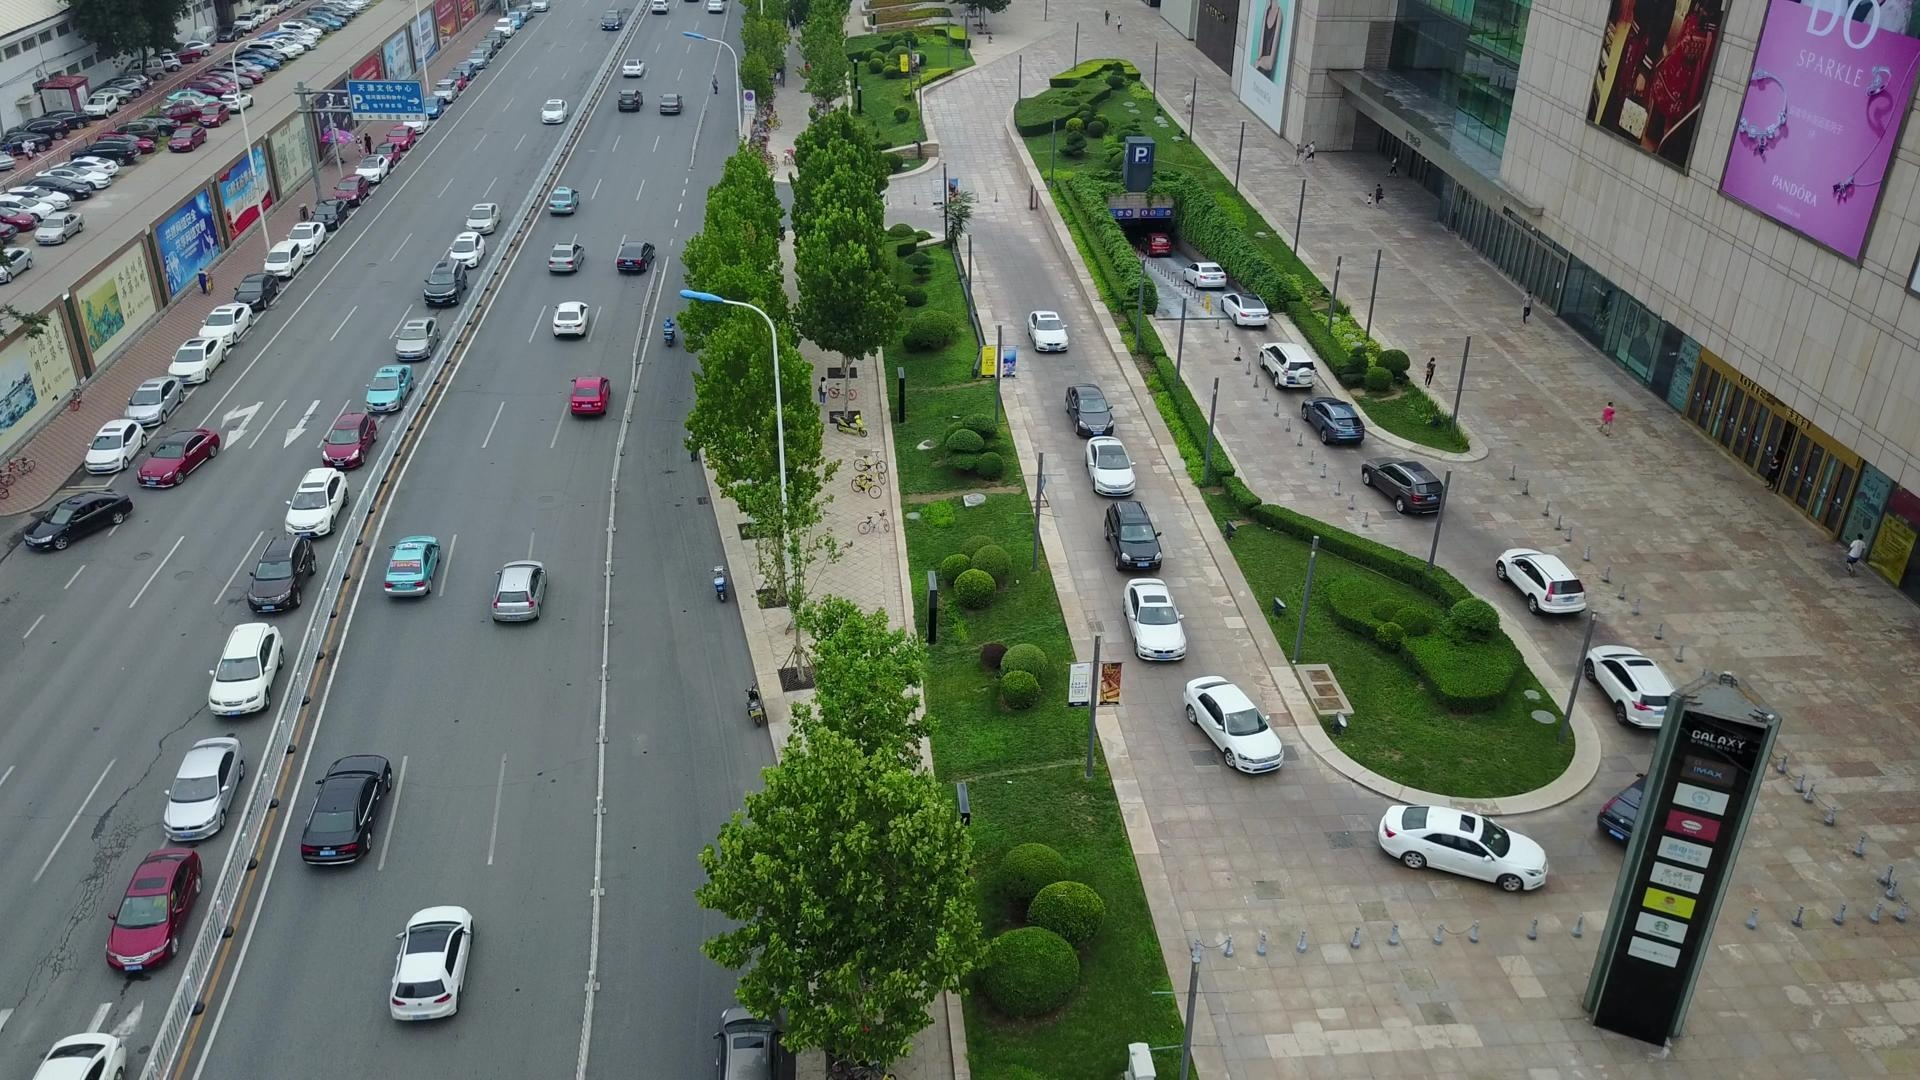
\includegraphics[
        width=8cm,
        height=8cm
    ]{sample_input.jpg}
};

%%%%%%%%%%%%%%%%%%%%%%%%%%%%%%%%%%%%%%%%%%%%%%%%%%%%%%%%%%%%%%%%%%%%%%%%%%%%%%%%%%%%%%%%
%% RESIZED IMAGE CORNERS
%%%%%%%%%%%%%%%%%%%%%%%%%%%%%%%%%%%%%%%%%%%%%%%%%%%%%%%%%%%%%%%%%%%%%%%%%%%%%%%%%%%%%%%%
%% helper coordinates for resize projection lines
%%%%%%%%%%%%%%%%%%%%%%%%%%%%%%%%%%%%%%%%%%%%%%%%%%%%%%%%%%%%%%%%%%%%%%%%%%%%%%%%%%%%%%%%

\coordinate (resize-nw) at (0.20,  4.00, -4.00);
\coordinate (resize-ne) at (0.20,  4.00,  4.00);
\coordinate (resize-sw) at (0.20, -4.00, -4.00);
\coordinate (resize-se) at (0.20, -4.00,  4.00);

%%%%%%%%%%%%%%%%%%%%%%%%%%%%%%%%%%%%%%%%%%%%%%%%%%%%%%%%%%%%%%%%%%%%%%%%%%%%%%%%%%%%%%%%
%% RESIZED IMAGE LABEL
%%%%%%%%%%%%%%%%%%%%%%%%%%%%%%%%%%%%%%%%%%%%%%%%%%%%%%%%%%%%%%%%%%%%%%%%%%%%%%%%%%%%%%%%
%% label for normalized CNN input image
%%%%%%%%%%%%%%%%%%%%%%%%%%%%%%%%%%%%%%%%%%%%%%%%%%%%%%%%%%%%%%%%%%%%%%%%%%%%%%%%%%%%%%%%

\path
(resize-sw) -- (resize-se)
node[
    midway,
    below=0.05cm,
    sloped,
    align=center
]
{
    \bfseries ~resized input
};


%%%%%%%%%%%%%%%%%%%%%%%%%%%%%%%%%%%%%%%%%%%%%%%%%%%%%%%%%%%%%%%%%%%%%%%%%%%%%%%%%%%%%%%%
%% FEATURE EXTRACTION
%%%%%%%%%%%%%%%%%%%%%%%%%%%%%%%%%%%%%%%%%%%%%%%%%%%%%%%%%%%%%%%%%%%%%%%%%%%%%%%%%%%%%%%%
%% convolutional feature extraction blocks of the CNN
%% each block contains:
%%
%% - convolution
%% - batch normalization
%% - ReLU activation
%% - max pooling
%%%%%%%%%%%%%%%%%%%%%%%%%%%%%%%%%%%%%%%%%%%%%%%%%%%%%%%%%%%%%%%%%%%%%%%%%%%%%%%%%%%%%%%%

\draw [connection]
(input-east) -- node {\midarrow}
($(input-east)+(3.7,0,0)$);

%%%%%%%%%%%%%%%%%%%%%%%%%%%%%%%%%%%%%%%%%%%%%%%%%%%%%%%%%%%%%%%%%%%%%%%%%%%%%%%%%%%%%%%%
%% CONVOLUTION BLOCK 1
%%%%%%%%%%%%%%%%%%%%%%%%%%%%%%%%%%%%%%%%%%%%%%%%%%%%%%%%%%%%%%%%%%%%%%%%%%%%%%%%%%%%%%%%
%% first feature extraction stage
%% spatial size: 128 x 128
%%%%%%%%%%%%%%%%%%%%%%%%%%%%%%%%%%%%%%%%%%%%%%%%%%%%%%%%%%%%%%%%%%%%%%%%%%%%%%%%%%%%%%%%

% Conv1-Block
\pic[shift={(3.7,0,0)}] at (input-east)
{Box={name=cr1,
    caption=conv1,
    xlabel={{"32",""}},
    fill=\ConvColor,
    height=40,
    width=3,
    depth=40,
    showfaceright=0,
    showfacebottom=0,
    showfaceback=0,
    opacity=0.5
}};

% BN/ReLU-Band daneben
\pic[shift={(0,0,0)}] at (cr1-east)
{Box={name=cr1_bn,
    fill=\ConvReluColor,
    zlabel=~~128,
    opacity=0.75,
    height=40,
    width=1,
    depth=40,
    hideedgez=1,
    hideedgey=1,
    showfaceleft=0,
    showfacebottom=0,
    showfaceback=0
}};


\node[shift={(2.05cm,-5.35cm)}] at (input-west)
{\small 128};


%%%%%%%%%%%%%%%%%%%%%%%%%%%%%%%%%%%%%%%%%%%%%%%%%%%%%%%%%%%%%%%%%%%%%%%%%%%%%%%%%%%%%%%%
%% MAX POOLING 1
%%%%%%%%%%%%%%%%%%%%%%%%%%%%%%%%%%%%%%%%%%%%%%%%%%%%%%%%%%%%%%%%%%%%%%%%%%%%%%%%%%%%%%%%
%% spatial downsampling after first convolution block
%%%%%%%%%%%%%%%%%%%%%%%%%%%%%%%%%%%%%%%%%%%%%%%%%%%%%%%%%%%%%%%%%%%%%%%%%%%%%%%%%%%%%%%%

\pic[shift={(0.2,0,0)}] at (cr1-east)
{Box={name=p1,
    fill=\PoolColor,
    opacity=0.55,
    height=34,
    width=1,
    depth=34
}};

%%%%%%%%%%%%%%%%%%%%%%%%%%%%%%%%%%%%%%%%%%%%%%%%%%%%%%%%%%%%%%%%%%%%%%%%%%%%%%%%%%%%%%%%
%% CONNECTION TO CONVOLUTION BLOCK 2
%%%%%%%%%%%%%%%%%%%%%%%%%%%%%%%%%%%%%%%%%%%%%%%%%%%%%%%%%%%%%%%%%%%%%%%%%%%%%%%%%%%%%%%%

\draw [connection]
(p1-east) -- node {\midarrow}
($(p1-east)+(2.0,0,0)$);

%%%%%%%%%%%%%%%%%%%%%%%%%%%%%%%%%%%%%%%%%%%%%%%%%%%%%%%%%%%%%%%%%%%%%%%%%%%%%%%%%%%%%%%%
%% CONVOLUTION BLOCK 2
%%%%%%%%%%%%%%%%%%%%%%%%%%%%%%%%%%%%%%%%%%%%%%%%%%%%%%%%%%%%%%%%%%%%%%%%%%%%%%%%%%%%%%%%
%% second feature extraction stage
%% spatial size: 64 x 64
%%%%%%%%%%%%%%%%%%%%%%%%%%%%%%%%%%%%%%%%%%%%%%%%%%%%%%%%%%%%%%%%%%%%%%%%%%%%%%%%%%%%%%%%

% Conv2-Block
\pic[shift={(2.0,0,0)}] at (p1-east)
{Box={name=cr2,
    caption=conv2,
    xlabel={{"64",""}},
    fill=\ConvColor,
    height=34,
    width=3.7,
    depth=34,
    showfaceright=0,
    showfacebottom=0,
    showfaceback=0,
    opacity=0.5
}};


% BN/ReLU-Band daneben
\pic[shift={(0,0,0)}] at (cr2-east)
{Box={name=cr2_bn,
    fill=\ConvReluColor,
    opacity=0.75,
    zlabel=~~64,
    height=34,
    width=1,
    depth=34,
    hideedgez=1,
    hideedgey=1,
    showfaceleft=0,
    showfacebottom=0,
    showfaceback=0
}};

\node[shift={(5.35cm,-4.5cm)}] at (input-west)
{\small 64};


%%%%%%%%%%%%%%%%%%%%%%%%%%%%%%%%%%%%%%%%%%%%%%%%%%%%%%%%%%%%%%%%%%%%%%%%%%%%%%%%%%%%%%%%
%% MAX POOLING 2
%%%%%%%%%%%%%%%%%%%%%%%%%%%%%%%%%%%%%%%%%%%%%%%%%%%%%%%%%%%%%%%%%%%%%%%%%%%%%%%%%%%%%%%%
%% spatial downsampling after second convolution block
%%%%%%%%%%%%%%%%%%%%%%%%%%%%%%%%%%%%%%%%%%%%%%%%%%%%%%%%%%%%%%%%%%%%%%%%%%%%%%%%%%%%%%%%

\pic[shift={(0.2,0,0)}] at (cr2-east)
{Box={name=p2,
    fill=\PoolColor,
    opacity=0.55,
    height=28,
    width=1,
    depth=28
}};

\draw [connection]
(p2-east) -- node {\midarrow}
($(p2-east)+(2.0,0,0)$);

%%%%%%%%%%%%%%%%%%%%%%%%%%%%%%%%%%%%%%%%%%%%%%%%%%%%%%%%%%%%%%%%%%%%%%%%%%%%%%%%%%%%%%%%
%% CONVOLUTION BLOCK 3
%%%%%%%%%%%%%%%%%%%%%%%%%%%%%%%%%%%%%%%%%%%%%%%%%%%%%%%%%%%%%%%%%%%%%%%%%%%%%%%%%%%%%%%%
%% third feature extraction stage
%% spatial size: 32 x 32
%%%%%%%%%%%%%%%%%%%%%%%%%%%%%%%%%%%%%%%%%%%%%%%%%%%%%%%%%%%%%%%%%%%%%%%%%%%%%%%%%%%%%%%%

% Conv3-Block
\pic[shift={(2.0,0,0)}] at (p2-east)
{Box={name=cr3,
    caption=conv3,
    xlabel={{"128",""}},
    fill=\ConvColor,
    height=28,
    width=5,
    depth=28,
    showfaceright=0,
    showfacebottom=0,
    showfaceback=0,
    opacity=0.5
}};


% BN/ReLU-Band daneben
\pic[shift={(0,0,0)}] at (cr3-east)
{Box={name=cr3_bn,
    fill=\ConvReluColor,
    opacity=0.75,
    zlabel=~~32,
    height=28,
    width=1,
    depth=28,
    hideedgez=1,
    hideedgey=1,
    showfaceleft=0,
    showfacebottom=0,
    showfaceback=0
}};


\node[shift={(8.7cm,-3.65cm)}] at (input-west)
{\small 32};


%%%%%%%%%%%%%%%%%%%%%%%%%%%%%%%%%%%%%%%%%%%%%%%%%%%%%%%%%%%%%%%%%%%%%%%%%%%%%%%%%%%%%%%%
%% MAX POOLING 3
%%%%%%%%%%%%%%%%%%%%%%%%%%%%%%%%%%%%%%%%%%%%%%%%%%%%%%%%%%%%%%%%%%%%%%%%%%%%%%%%%%%%%%%%
%% spatial downsampling after third convolution block
%%%%%%%%%%%%%%%%%%%%%%%%%%%%%%%%%%%%%%%%%%%%%%%%%%%%%%%%%%%%%%%%%%%%%%%%%%%%%%%%%%%%%%%%

\pic[shift={(0.20,0,0)}] at (cr3-east)
{Box={name=p3,
    fill=\PoolColor,
    opacity=0.55,
    height=21,
    width=1,
    depth=21
}};

\draw [connection]
(p3-east) -- node {\midarrow}
($(p3-east)+(1.8,0,0)$);

%%%%%%%%%%%%%%%%%%%%%%%%%%%%%%%%%%%%%%%%%%%%%%%%%%%%%%%%%%%%%%%%%%%%%%%%%%%%%%%%%%%%%%%%
%% CONVOLUTION BLOCK 4
%%%%%%%%%%%%%%%%%%%%%%%%%%%%%%%%%%%%%%%%%%%%%%%%%%%%%%%%%%%%%%%%%%%%%%%%%%%%%%%%%%%%%%%%
%% final convolutional feature extraction stage
%% spatial size: 16 x 16
%%%%%%%%%%%%%%%%%%%%%%%%%%%%%%%%%%%%%%%%%%%%%%%%%%%%%%%%%%%%%%%%%%%%%%%%%%%%%%%%%%%%%%%%

% Conv4-Block
\pic[shift={(1.8,0,0)}] at (p3-east)
{Box={name=cr4,
    caption=conv4,
    xlabel={{"128",""}},
    fill=\ConvColor,
    height=21,
    width=5,
    depth=21,
    showfaceright=0,
    showfacebottom=0,
    showfaceback=0,
    opacity=0.5
}};


% BN/ReLU-Band daneben
\pic[shift={(0,0,0)}] at (cr4-east)
{Box={name=cr4_bn,
    fill=\ConvReluColor,
    opacity=0.75,
    zlabel=~~16,
    height=21,
    width=0.8,
    depth=21,
    hideedgez=1,
    hideedgey=1,
    showfaceleft=0,
    showfacebottom=0,
    showfaceback=0
}};

\node[shift={(12.15cm,-2.7cm)}] at (input-west)
{
    \small 16
};


%%%%%%%%%%%%%%%%%%%%%%%%%%%%%%%%%%%%%%%%%%%%%%%%%%%%%%%%%%%%%%%%%%%%%%%%%%%%%%%%%%%%%%%%
%% CLASSIFICATION HEAD
%%%%%%%%%%%%%%%%%%%%%%%%%%%%%%%%%%%%%%%%%%%%%%%%%%%%%%%%%%%%%%%%%%%%%%%%%%%%%%%%%%%%%%%%
%% converts extracted feature maps into compact feature vectors
%% and predicts one of the six degradation classes
%%%%%%%%%%%%%%%%%%%%%%%%%%%%%%%%%%%%%%%%%%%%%%%%%%%%%%%%%%%%%%%%%%%%%%%%%%%%%%%%%%%%%%%%

\draw [connection]
(cr4_bn-east) -- node {\midarrow}
($(cr4-east)+(2.0,0,0)$);

%%%%%%%%%%%%%%%%%%%%%%%%%%%%%%%%%%%%%%%%%%%%%%%%%%%%%%%%%%%%%%%%%%%%%%%%%%%%%%%%%%%%%%%%
%% GLOBAL AVERAGE POOLING
%%%%%%%%%%%%%%%%%%%%%%%%%%%%%%%%%%%%%%%%%%%%%%%%%%%%%%%%%%%%%%%%%%%%%%%%%%%%%%%%%%%%%%%%
%% reduces feature maps into compact 1 x 1 feature representation
%%%%%%%%%%%%%%%%%%%%%%%%%%%%%%%%%%%%%%%%%%%%%%%%%%%%%%%%%%%%%%%%%%%%%%%%%%%%%%%%%%%%%%%%

% Global Average Pooling
\pic[shift={(2.0,0,0)}] at (cr4-east)
{Box={name=gap,
    caption=global avg pool,
    xlabel={{"128",""}},
    zlabel=~~1,
    fill=\GapColor,
    opacity=0.9,
    height=5,
    width=14.75,
    depth=5
}};

\node[shift={(15.9cm,-0.5cm)}] at (input-west)
{
    \small 1
};

\node[shift={(19.85cm,-0.4cm)}] at (input-west)
{
    \small 1
};


\node[shift={(23.85cm,-0.3cm)}] at (input-west)
{
    \small 1
};


%%%%%%%%%%%%%%%%%%%%%%%%%%%%%%%%%%%%%%%%%%%%%%%%%%%%%%%%%%%%%%%%%%%%%%%%%%%%%%%%%%%%%%%%
%% CONNECTION TO DENSE LAYER
%%%%%%%%%%%%%%%%%%%%%%%%%%%%%%%%%%%%%%%%%%%%%%%%%%%%%%%%%%%%%%%%%%%%%%%%%%%%%%%%%%%%%%%%

\draw [connection]
(gap-east) -- node {\midarrow}
($(gap-east)+(1.0,0,0)$);

%%%%%%%%%%%%%%%%%%%%%%%%%%%%%%%%%%%%%%%%%%%%%%%%%%%%%%%%%%%%%%%%%%%%%%%%%%%%%%%%%%%%%%%%
%% DENSE CLASSIFICATION LAYER
%%%%%%%%%%%%%%%%%%%%%%%%%%%%%%%%%%%%%%%%%%%%%%%%%%%%%%%%%%%%%%%%%%%%%%%%%%%%%%%%%%%%%%%%
%% fully connected classification layer with 128 neurons
%%%%%%%%%%%%%%%%%%%%%%%%%%%%%%%%%%%%%%%%%%%%%%%%%%%%%%%%%%%%%%%%%%%%%%%%%%%%%%%%%%%%%%%%

% Dense-Block
\draw [connection]
(gap-east) -- node {\midarrow}
($(gap-east)+(1.0,0,0)$);

\pic[shift={(1.0,0,0)}] at (gap-east)
{Box={name=fc,
    caption=dense 128,
    xlabel={"128",""},
    fill=\SoftmaxColor,
    height=4,
    width=14,
    depth=4,
    showfaceright=0,
    showfacebottom=0,
    showfaceback=0
}};

%%%%%%%%%%%%%%%%%%%%%%%%%%%%%%%%%%%%%%%%%%%%%%%%%%%%%%%%%%%%%%%%%%%%%%%%%%%%%%%%%%%%%%%%
%% RELU ACTIVATION BAND
%%%%%%%%%%%%%%%%%%%%%%%%%%%%%%%%%%%%%%%%%%%%%%%%%%%%%%%%%%%%%%%%%%%%%%%%%%%%%%%%%%%%%%%%
%% separate activation band placed next to dense layer
%%%%%%%%%%%%%%%%%%%%%%%%%%%%%%%%%%%%%%%%%%%%%%%%%%%%%%%%%%%%%%%%%%%%%%%%%%%%%%%%%%%%%%%%

% ReLU-Band daneben
\pic[shift={(0,0.0,0)}] at (fc-east)
{Box={name=fc_relu,
    fill=\ConvReluColor,
    opacity=0.75,
    zlabel=~~1,
    height=4,
    width={0.75},
    depth=4,
    hideedgez=1,
    hideedgey=1,
    showfaceleft=0,
    showfacebottom=0,
    showfaceback=0
}};

%%%%%%%%%%%%%%%%%%%%%%%%%%%%%%%%%%%%%%%%%%%%%%%%%%%%%%%%%%%%%%%%%%%%%%%%%%%%%%%%%%%%%%%%
%% DROPOUT VISUALIZATION
%%%%%%%%%%%%%%%%%%%%%%%%%%%%%%%%%%%%%%%%%%%%%%%%%%%%%%%%%%%%%%%%%%%%%%%%%%%%%%%%%%%%%%%%
%% dropout is visualized as dotted overlay on activation band
%% to keep the architecture compact but still visually interpretable
%%%%%%%%%%%%%%%%%%%%%%%%%%%%%%%%%%%%%%%%%%%%%%%%%%%%%%%%%%%%%%%%%%%%%%%%%%%%%%%%%%%%%%%%

% Dropout dot pattern overlay on ReLU block
\draw[
    pattern=crosshatch dots,
    pattern color=red!60!black
]
(fc_relu-nearnorthwest) --
(fc_relu-nearnortheast) --
(fc_relu-nearsoutheast) --
(fc_relu-nearsouthwest) -- cycle;

\draw[
    pattern=crosshatch dots,
    pattern color=red!60!black
]
(fc_relu-farnorthwest) --
(fc_relu-farnortheast) --
(fc_relu-nearnortheast) --
(fc_relu-nearnorthwest) -- cycle;

\draw[
    pattern=crosshatch dots,
    pattern color=red!60!black
]
(fc_relu-nearnortheast) --
(fc_relu-farnortheast) --
(fc_relu-farsoutheast) --
(fc_relu-nearsoutheast) -- cycle;

%%%%%%%%%%%%%%%%%%%%%%%%%%%%%%%%%%%%%%%%%%%%%%%%%%%%%%%%%%%%%%%%%%%%%%%%%%%%%%%%%%%%%%%%
%% OUTPUT LAYER
%%%%%%%%%%%%%%%%%%%%%%%%%%%%%%%%%%%%%%%%%%%%%%%%%%%%%%%%%%%%%%%%%%%%%%%%%%%%%%%%%%%%%%%%
%% final dense output block for six degradation classes
%%%%%%%%%%%%%%%%%%%%%%%%%%%%%%%%%%%%%%%%%%%%%%%%%%%%%%%%%%%%%%%%%%%%%%%%%%%%%%%%%%%%%%%%

% Output-Block
\draw [connection]
(fc_relu-east) -- node {\midarrow}
($(fc_relu-east)+(1.1,0,0)$);

\pic[shift={(1,0,0)}] at (fc_relu-east)
{Box={name=out,
    caption=output,
    xlabel={"6"},
    fill=\SoftmaxColor,
    height=4,
    width=1.7,
    depth=4,
    showfaceright=0,
    showfacebottom=0,
    showfaceback=0
}};

%%%%%%%%%%%%%%%%%%%%%%%%%%%%%%%%%%%%%%%%%%%%%%%%%%%%%%%%%%%%%%%%%%%%%%%%%%%%%%%%%%%%%%%%
%% SOFTMAX BAND
%%%%%%%%%%%%%%%%%%%%%%%%%%%%%%%%%%%%%%%%%%%%%%%%%%%%%%%%%%%%%%%%%%%%%%%%%%%%%%%%%%%%%%%%
%% softmax activation for class probability output
%%%%%%%%%%%%%%%%%%%%%%%%%%%%%%%%%%%%%%%%%%%%%%%%%%%%%%%%%%%%%%%%%%%%%%%%%%%%%%%%%%%%%%%%

% Softmax-Band daneben
\pic[shift={(0,0,0)}] at (out-east)
{Box={name=out_softmax,
    fill=\SoftmaxBandColor,
    opacity=0.75,
    zlabel=~~1,
    height=4,
    width=0.5,
    depth=4,
    hideedgez=1,
    hideedgey=1,
    showfaceleft=0,
    showfacebottom=0,
    showfaceback=0
}};

\draw [connection] (out_softmax-east) -- node {\midarrow} ++(1,0,0);

%%%%%%%%%%%%%%%%%%%%%%%%%%%%%%%%%%%%%%%%%%%%%%%%%%%%%%%%%%%%%%%%%%%%%%%%%%%%%%%%%%%%%%%%
%% PREDICTION OUTPUT BOX
%%%%%%%%%%%%%%%%%%%%%%%%%%%%%%%%%%%%%%%%%%%%%%%%%%%%%%%%%%%%%%%%%%%%%%%%%%%%%%%%%%%%%%%%
%% final visual output of the CNN prediction pipeline
%%%%%%%%%%%%%%%%%%%%%%%%%%%%%%%%%%%%%%%%%%%%%%%%%%%%%%%%%%%%%%%%%%%%%%%%%%%%%%%%%%%%%%%%

\coordinate (prediction-box-pos) at (out_softmax-east);

\node[
    draw,
    rounded corners=3pt,
    thick,
    minimum width=3.7cm,
    minimum height=1.3cm,
    fill=PredictionGreen,
    opacity=0.95,
    text opacity=1,
    align=center,
    right=1cm of out_softmax-east
]
{
    \bfseries predicted\\
    \bfseries degradation class
};


%%%%%%%%%%%%%%%%%%%%%%%%%%%%%%%%%%%%%%%%%%%%%%%%%%%%%%%%%%%%%%%%%%%%%%%%%%%%%%%%%%%%%%%%
%% FEATURE MAP -> VECTOR TRANSITION
%%%%%%%%%%%%%%%%%%%%%%%%%%%%%%%%%%%%%%%%%%%%%%%%%%%%%%%%%%%%%%%%%%%%%%%%%%%%%%%%%%%%%%%%
%% dashed lines show the transition from spatial feature maps
%% to compact feature vector representation
%%%%%%%%%%%%%%%%%%%%%%%%%%%%%%%%%%%%%%%%%%%%%%%%%%%%%%%%%%%%%%%%%%%%%%%%%%%%%%%%%%%%%%%%

\draw[densely dashed, opacity=0.45]
    (gap-nearnorthwest) -- (cr4_bn-nearnortheast)
    (gap-nearsouthwest) -- (cr4_bn-nearsoutheast)
    (gap-farsouthwest)  -- (cr4_bn-farsoutheast)
    (gap-farnorthwest)  -- (cr4_bn-farnortheast);

%%%%%%%%%%%%%%%%%%%%%%%%%%%%%%%%%%%%%%%%%%%%%%%%%%%%%%%%%%%%%%%%%%%%%%%%%%%%%%%%%%%%%%%%
%% RESIZE PROJECTION LINES
%%%%%%%%%%%%%%%%%%%%%%%%%%%%%%%%%%%%%%%%%%%%%%%%%%%%%%%%%%%%%%%%%%%%%%%%%%%%%%%%%%%%%%%%
%% dashed lines connect original image size with resized CNN input
%%%%%%%%%%%%%%%%%%%%%%%%%%%%%%%%%%%%%%%%%%%%%%%%%%%%%%%%%%%%%%%%%%%%%%%%%%%%%%%%%%%%%%%%

\draw[densely dashed, opacity=0.45]
    (resize-nw) -- (raw-nw)
    (resize-ne) -- (raw-ne)
    (resize-sw) -- (raw-sw)
    (resize-se) -- (raw-se);

\path
(raw-se) -- (resize-se)
node[
    midway,
    below=0.1cm,
    sloped,
    opacity=1,
    align=center
]
{
    \bfseries Resizing of input images:\\
    \ original input size normalized\\
      to 128 $\times$ 128 RGB
};

%%%%%%%%%%%%%%%%%%%%%%%%%%%%%%%%%%%%%%%%%%%%%%%%%%%%%%%%%%%%%%%%%%%%%%%%%%%%%%%%%%%%%%%%
%% TITLE
%%%%%%%%%%%%%%%%%%%%%%%%%%%%%%%%%%%%%%%%%%%%%%%%%%%%%%%%%%%%%%%%%%%%%%%%%%%%%%%%%%%%%%%%
%% main title of the CNN architecture visualization
%%%%%%%%%%%%%%%%%%%%%%%%%%%%%%%%%%%%%%%%%%%%%%%%%%%%%%%%%%%%%%%%%%%%%%%%%%%%%%%%%%%%%%%%

\node[
    font=\bfseries\fontsize{22}{26}\selectfont,
    align=center
] at (12,7.9)
{
    CNN-Based Image Quality Classifier\\
};


%%%%%%%%%%%%%%%%%%%%%%%%%%%%%%%%%%%%%%%%%%%%%%%%%%%%%%%%%%%%%%%%%%%%%%%%%%%%%%%%%%%%%%%%
%% LEGEND - CNN ARCHITECTURE
%%%%%%%%%%%%%%%%%%%%%%%%%%%%%%%%%%%%%%%%%%%%%%%%%%%%%%%%%%%%%%%%%%%%%%%%%%%%%%%%%%%%%%%%
%% explains visual meaning of colors, blocks and arrows
%% used in the architecture diagram
%%%%%%%%%%%%%%%%%%%%%%%%%%%%%%%%%%%%%%%%%%%%%%%%%%%%%%%%%%%%%%%%%%%%%%%%%%%%%%%%%%%%%%%%

% --------------------------------------------------
% ReLU + Dropout
% --------------------------------------------------

\fill[
    fill=\ConvReluColor,
    opacity=0.75
]
(11.8,-6.9) rectangle (12.8,-6.1);

\fill[
    pattern=crosshatch dots,
    pattern color=red!60!black
]
(11.8,-6.9) rectangle (12.8,-6.1);

\node[
    anchor=west,
    align=left
] at (12.9,-6.5)
{
    \small ReLU activation\\
    \small + 0.4 dropout
};

% ==================================================
% COLUMN 0 - FLOW
% ==================================================

% --------------------------------------------------
% Forward data flow
% --------------------------------------------------

\draw[
    connection
]
(11.8,-8.0) -- node {\midarrow} (13.0,-8.0);

\node[
    anchor=west,
    align=left
] at (13.1,-8.0)
{
    \small forward data flow
};


% ==================================================
% COLUMN 1 - FEATURE EXTRACTION
% ==================================================

% --------------------------------------------------
% Convolution
% --------------------------------------------------

\fill[
    fill=\ConvColor,
    opacity=0.5
]
(17.8,-5.4) rectangle (18.8,-4.6);

\node[
    anchor=west,
    align=left
] at (18.9,-5.0)
{
    \small convolutional layer\\
    \small + batch normalisation
};


% --------------------------------------------------
% ReLU activation
% --------------------------------------------------

\fill[
    fill=\ConvReluColor,
    opacity=0.75
]
(17.8,-6.9) rectangle (18.8,-6.1);

\node[
    anchor=west,
    align=left
] at (18.9,-6.5)
{
    \small ReLU activation
};


% --------------------------------------------------
% Max Pooling
% --------------------------------------------------

% Hintergrund (ReLU-Farbe)

\fill[
    fill=\ConvReluColor,
    opacity=0.75
]
(17.8,-8.4) rectangle (18.8,-7.6);

% Vordergrund (Pooling-Farbe)

\fill[
    fill=\PoolColor,
    opacity=0.55
]
(17.8,-8.4) rectangle (18.8,-7.6);

\node[
    anchor=west,
    align=left
] at (18.9,-8.0)
{
    \small max pooling\\
    \small for spatial downsampling
};


% ==================================================
% COLUMN 2 - CLASSIFICATION
% ==================================================

% --------------------------------------------------
% Global Average Pooling
% --------------------------------------------------

\fill[
    fill=\GapColor,
    opacity=0.9
]
(23.8,-5.4) rectangle (24.8,-4.6);

\node[
    anchor=west,
    align=left
] at (24.9,-5.0)
{
    \small global average pooling\\
    \small for feature vector generation
};


% --------------------------------------------------
% Dense Layer
% --------------------------------------------------

\fill[
    fill=\SoftmaxColor,
    opacity=0.4
]
(23.8,-6.9) rectangle (24.8,-6.1);

\node[
    anchor=west,
    align=left
] at (24.9,-6.5)
{
    \small dense layer
};


% --------------------------------------------------
% Softmax
% --------------------------------------------------

\fill[
    fill=\SoftmaxColor,
    opacity=0.4
]
(23.8,-8.4) rectangle (24.8,-7.6);

\fill[
    fill=\SoftmaxBandColor,
    opacity=0.75
]
(23.8,-8.4) rectangle (24.8,-7.6);

\node[
    anchor=west,
    align=left
] at (24.9,-8.0)
{
    \small softmax activation\\
    \small for class probabilities
};

%%%%%%%%%%%%%%%%%%%%%%%%%%%%%%%%%%%%%%%%%%%%%%%%%%%%%%%%%%%%
\end{tikzpicture}
\end{document}
